\chapter{Implementation and API}
In this chapter we will present implementation details of our system. First we present all libraries used in this project. Later we will introduce outcome in form of \gls{ROS} package. We will briefly introduce structure of the program and key components.
\section{Used libraries}
\section {\gls{ROS}}
The \gls{ROS} \cite{ros_papper} is popular robotic framework. It offers flexible way how to combine existing tools, libraries and algorithms to make full robotic solution from sensor drivers up to higher logic of planning and mapping. A communication between individual programs (nodes) is done through subscriber-publisher model. A configuration of programs is saved in parameter server. This server also take care of managing communication between two nodes.  
\subsection{The Point Cloud library}
The \gls{PCL} is a standard \gls{ROS} library for manipulation with point clouds \cite{pcl}. The library includes state-of-the-art algorithms in registration, filtering, segmentation and feature extraction. It contains also tools for visualization and manipulation with point clouds. In our project we used mostly base point cloud datastructure for exchange of point cloud data inside of algorithm. We have also used registration base class for implementation of our scan matching algorithms. 
\subsection{The G2O}
The G2O is pose graph optimization library presented by \cite{g2o}. It is currently the most used library for pose graph optimization. It offers well designed extendable interface. It is relatively easy to add new definition of pose graph optimization. New optimization methods often have version of the algorithm included into this library. In our program it is used as main optimization engine for pose graph.
\subsection{The Eigen}
The Eigen \cite{eigenweb} is templated C++ library for linear algebra. It includes modules for dense and sparse matrix representations, numerical solvers, transformation representation. This project mostly uses geometry module with affine transformation. We also utilize numerical solvers in our implementation of registration algorithms. We have selected this library, because it is considered standard library for linear algebra in \gls{ROS}. Many packages use it and offer API's designed with this library components.   
\section{ROS package}
This work provides single \gls{ROS} package NDT-GSLAM2D implemented in C++11. This package offers standard \gls{ROS} interface for mapping and localizing algorithms. Full documentation of this interface is in Appendix \ref{chap:ndt_gslam_package}. 

Expected input data for \gls{SLAM} algorithms in \gls{ROS} is using laser message. It is also possible to provide odometry information for our algorithm. This is not a requirement, but algorithm can utilize if iser provide good source of robot movement information. Our goal was to extend this interface in a way which will make it easy to use. We have noticed that many packages in \gls{ROS} do not cover all possible input data. This makes users built wrappers around original packages. During our design process we have decided to also allow substituting laser message by point cloud. The point clouds are standard in 3D mapping and it is reasonable to expect them also in 2D variant. Our implementation also include full configuration for subscribe and publish topics. This makes it easy to use package using nonstandard topics.  
\section{Structure of the system}
Architecture of the whole system can be divided into 3 parts. The first part is already mentioned \gls{ROS} interface. The second part is main algorithms C++ interface mapping all data to and from \gls{ROS} node. We decided to have this double interface, because it is convenient to use algorithm also without \gls{ROS} interface. This was mainly used for debugging and testing purposes. It is also convenient representation if we decide to do second adaptation of our algorithm. In this case, we do not have to rewrite node's source code. In this layer of abstraction we take care of initial estimation of odometry and \gls{NDT} frame building process. A map generation and updates also take place in this part of architecture.

Thirds part is graph \gls{SLAM} interface. This interface makes abstraction around graph creation and optimization process. This section is using our custom pose graph implementation. On top of this graph we developed loop closure detection and validation. This graph is synchronized with the graph inside of optimization engine G2O. We carry two graphs for reason of easier switching between different optimization engines in the future. Our graph representation also include additional information about state and type of edge. Implementing it into G2O would require rewrite this code with every new optimizer.

Important part of architecture is handling of \gls{NDT} frames. A created frame is held inside shared pointer. The same pattern is used in \gls{PCL}'s point cloud data type. The shared pointer is then passed to the graph creation process and also to \gls{NDT} map building process. Nodes of the pose graph include this pointer as their representation of the world. \gls{NDT} frames in nodes are used for loop closure registration. This means that registration algorithm use the constant shared pointers as well. This is also standard registration algorithm behavior in \gls{PCL}. 
 
 \begin{figure}
 	\centering
 	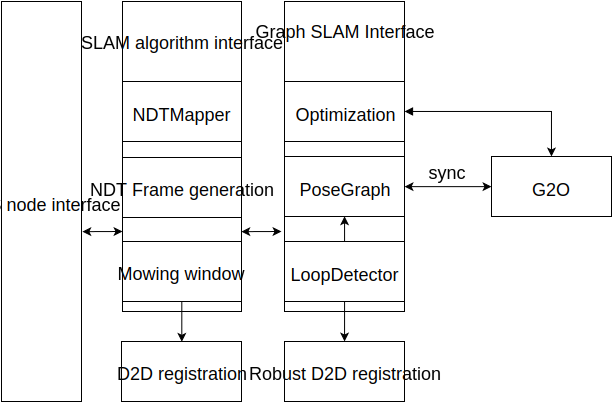
\includegraphics[width=140mm]{../img/architecture.png}
 	\caption{Overview of individual parts of architecture and their relationships.}\label{fig:architecture}
 \end{figure}
      
\section{NDTGrid2D}
The NDTGrid2D is the main class for all operations in our approach. It offers basic functionality for grid creation. It can be merged with or without use of ray-tracing. It is used for dynamic entity update from \gls{NDT-OM}. It also offers grid translation which is needed for moving window. Another group of functionality is for registration algorithms. They require radius search and k-nearest neighbor search. Odometry estimator also needs to use means from cells. The last group is output format methods. Grid is able to create coarser instance of itself. It is also able to be printed to standard console output. We have implemented methods for conversion into our custom type of occupancy and \gls{NDT} map messages. These messages are used only internally and later can be transformed into \gls{ROS} variants.

In order to fulfill all these needs implementation of NDTGrid2D is just a higher abstraction layer on top of VoxelGrid2D. The voxel grid is taking care of memory layout, resizing, element lookup and ray-tracing. The NDTGrid2D has two template parameters. The first parameter is type of the cell. Grid is initialized from point cloud, for this reason it needs to have second template parameter for type of point. This is standard approach in \gls{PCL} related algorithms.  

Core algorithm logic for merging and updating cells is stored inside every cell. This allows developing new cells without any changes to the grid.
\subsection{VoxelGrid2D}
It is general grid like structure with one template parameter. The type used in class is requires to have implemented only  operator plus and copy constructor. This datastracture is intended to use with larger cell types in sparse environment. Based on these requirements it holds pointers to all cells. In case of unoccupied cell it uses null pointers. The grid is initialized empty with no cells inside. Based on addition process it dynamically resize the grid. It also has method for manual resizing which makes memory allocation efficient. It offers base functionality for ray-tracing and radius search. Incoming cells may be added to previous data in cell or just replace old content.  
\subsection{NDTCell}
The \gls{NDT} cell is the core of all calculations on top of the grid. In case of \gls{NDT-OM} implementation it holds covariance and mean estimation, occupancy update rule and \gls{RCU} update rule for merging of cells with Gaussian inside. In the future experiments we can easily design new type of cell based on current algorithm requirements and keep NDTGrid2D and the VoxelGrid without modifications.
\section{Registration algorithms}
When designing registration algorithms we have decided to use same interface as \gls{PCL}'s registration algorithms. By extension of their base class our programs can be used standard way inside of \gls{PCL}. This makes it easy to use our algorithms alongside \gls{PCL}  implementations. It also possible to use all visualization and io tools provided by \gls{PCL}. 

